\input{Packages}
\input{Definitions}
\DeclareRobustCommand{\stirling}{\genfrac\{\}{0pt}{}}
%this removes numbering from the section, from some reason the \section*{} command doesnt work once you redefine it
\setcounter{secnumdepth}{0} 

% Define variables for week number and meeting date
\newcommand{\weekNum}{9} % Change this to update the week number
\newcommand{\meetingDate}{Mar 19, 2025} 

\usepackage{pgfplots}
\pgfplotsset{compat=1.17}

\begin{document}
\pagestyle{empty}
\sloppy
\maketitle

\section{Topic: Invariants, Monovariants, \& Constructions}

\begin{problem}[C][2][Arthur Engel, Problem Solving Strategies]
    %Discrete ^ Invariants
    An $8\times8$ chessboard is colored in the usual way, but that’s boring, so you decide to fix this. You can take any row, column, or $2\times2$ square, and reverse the colors inside it, switching black to white and white to black.\\[\parskip]
    
    Prove that it’s impossible to end up with 63 white squares and 1 black square.
\end{problem}

\begin{solution}
    If we try reaching 1 black tile a few different times, we find that no matter what we do, we are unable to achieve it. What we notice instead is that we always end up with an even number of black tiles---this appears to be the key invariant property, and, if true, proves that reaching just 1 black tile alone is impossible. 

    To show that we always have an even number of black squares, we point out that, to start, we obviously have an even number of black squares. Now, we show that we are always adding or subtracting an even number of black squares, so the count remains even. Looking at the $2\times2$ square transformation, we see that if we start from 0, 1, 2, 3, or 4 black squares, we end up with 4, 3, 2, 1, or 0 black squares respectively, resulting in an even change in the number of black squares each time. 
    \begin{center}
    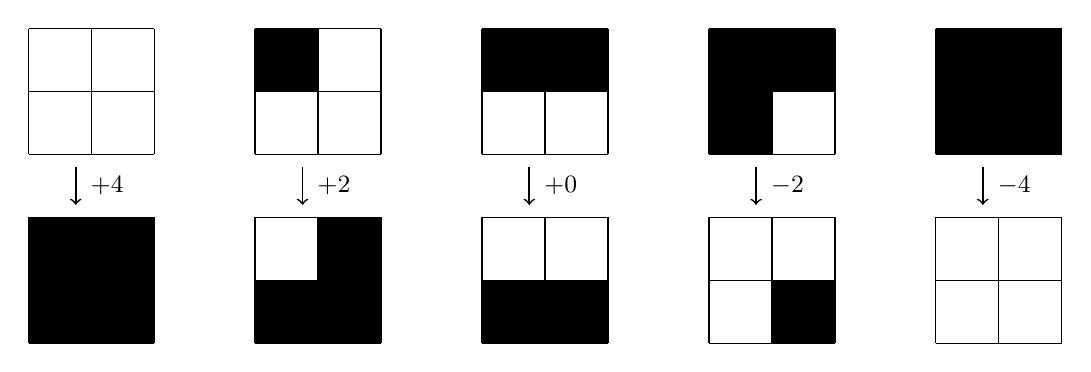
\begin{tikzpicture}[scale=0.8]
        \def\xsep{3.6}
        \def\ysep{3}
    
        \foreach \i/\w/\x/\y/\z in {0/0/0/0/0, 1/1/0/0/0, 2/1/1/0/0, 3/1/1/1/0, 4/1/1/1/1} {
            \pgfmathsetmacro{\xshift}{\i * \xsep}
            \pgfmathsetmacro{\D}{4-2*\i}
            \begin{scope}[xshift=\xshift cm]
                \fill[white] (0,0) rectangle (2,2);
                \draw[semithick] (0,0) grid (2,2);
    
                \ifnum\w=1
                    \fill[black] (0,1) rectangle ++(1,1);
                \fi
                \ifnum\x=1
                    \fill[black] (1,1) rectangle ++(1,1);
                \fi
                \ifnum\y=1
                    \fill[black] (0,0) rectangle ++(1,1);
                \fi
                \ifnum\z=1
                    \fill[black] (1,0) rectangle ++(1,1);
                \fi
    
                \draw[semithick, ->] (0.75,-0.2) -- (0.75,-0.8);
                \node at (1.25, -0.5) {\small $\pgfmathprintnumber[print sign, precision=0]{\D}$};
            \end{scope}
    
            \begin{scope}[yshift=-\ysep cm, xshift=\xshift cm]
                \fill[white] (0,0) rectangle (2,2);
                \draw[semithick] (0,0) grid (2,2);
    
                \ifnum\w=0
                    \fill[black] (0,1) rectangle ++(1,1);
                \fi
                \ifnum\x=0
                    \fill[black] (1,1) rectangle ++(1,1);
                \fi
                \ifnum\y=0
                    \fill[black] (0,0) rectangle ++(1,1);
                \fi
                \ifnum\z=0
                    \fill[black] (1,0) rectangle ++(1,1);
                \fi
            \end{scope}
        }
    \end{tikzpicture}
    \end{center}
    
    We'll generalize this a bit for the other transformations. For a given row/column with $B$ black tiles, there are $8-B$ white tiles. After the flip, $8-B$ black tiles are added and $B$ black tiles are lost, for a change of $8-2B$ black tiles, which is again an even number regardless of $B$. Thus, in every case, we only add or subtract an even number of black tiles, meaning it's impossible to end up with just 1 of them.
\end{solution}

\begin{problem}[C][2][BmMT 2015 Individual/2]
    %Counting
    In Fourtown, every person must have a car and therefore a license plate. Every license plate must be a 4-digit number where each digit is a value between 0 and 9 inclusive. However 0000 is not a valid license plate. What is the minimum population of Fourtown to guarantee that at least two people have the same license plate?
\end{problem}

\begin{solution}
    The smallest license plate number is $0001$ and the largest is $9999$, for a total of $9999$ possible license plates. Thus, by the Pigeonhole Principle, there must be $\boxed{10000}$ people in Fourtown to gaurentee at least one duplicate license plate.
\end{solution}


%this one is easier so i moved it up -- edgar
\begin{problem}[C][3]
    %Discrete ^ Pigeon-Hole Principle
    Show that if we select 5 points inside a square of length $1$, there are at least two points who are at most $\sqrt{2}/2$ apart.
\end{problem}

\begin{solution}
    Join the middle points of the square to create four equal squares of length $1/2$. Since we are selecting five points, it follows from the Pigeon-Hole Principle that at least two points are contained within the same square. Where the maximum distance that can exist between them is the length of the diagonal: $\ \sqrt 2 / 2$ $\Box$
\end{solution}

\begin{problem}[C][4][Problem Solving Seminar, Hough and Vakil/3]
    %Discrete ^ Monovariants ^ Invariants
    N cats and N dogs are distributed among the rooms of a mansion. They move among the rooms according to the rules: either  

    {\raggedright\begin{itemize}[topsep=2mm, itemsep=1mm]
        \item a cat moves from a room with more cats than dogs (counted before it moves) into a room with more dogs than cats, or  
        \item a dog moves from a room with more dogs than cats into a room with more cats than dogs.
    \end{itemize}}

    Show that, eventually, the cats and dogs will stop moving. 
\end{problem}

\begin{solution} 
    Let $k$ be the number of rooms of the mansion. For $1 \leq i \leq k$, denote $a_i, b_i$ as the amount of dogs and cats in room $i$, respectively. 
    Where we know $a_1 + a_2 + \ldots +a_k = b_1 + b_2 + \ldots + b_k = N $. Define
    $$S = |a_1 - b_1| + |a_2 - b_2| + \ldots + |a_k - b_k|$$
    We claim that $S$ is even, because we know $a \equiv -a \pmod 2 \iff |a| \equiv a \pmod 2$ for any integer $a$. We deduce  that 
    $$S \equiv a_1 - b_1 + a_2 - b_2 + \ldots + a_k - b_k = N - N = 0 \pmod 2$$
    Back to the problem, let $s_i = |a_i - b_i|$ for $1 \leq i \leq k$, it is easy to see that $S = s_1 + s_2 + \ldots + s_k$. We will show that we eventually have $S=0$, and because $s_i \geq 0$, this would imply $s_i=0 \Rightarrow a_i = b_i$ and therefore the cats and dogs would stop moving.

    If a dog moves from room $u$ to room $v$, it is because $a_u > b_u$ and $a_v < b_v$, this means that $s_u = a_u - b_u$ and $s_v = b_v - a_v$. Because the dog moved, both $s_u$ and $s_v$ decreased by 1, thus $S$ decreased by $2$. The same argument can be applied for a cat as well.

    Now, because $S$ is always even, nonnegative, and it is decreased by $2$ after each move, we conclude that we eventually reach $S = 0$. $\Box$
    
\end{solution}
 
\begin{problem}[C][4][Western PA ARML Practice/4]
    %Discrete ^ Invariants
    At a party, some pairs of people shake hands. We call a person \emph{odd} if they have shaken hands with an odd number of other guests. Prove that there is an even number of odd people at the party.
\end{problem}

\begin{solution}
    Consider possible pairs of people that could shake hands. Either both people are odd, only 1 person is odd, or neither of them are odd. Then consider that whenever an odd person shakes hands with someone new, they become even. And when an even person shakes hands with someone new, they become odd. Now, observe how the overall number of odd people $N$ changes in each case---this change is always an even amount:
    \begin{alignat*}{6}
        (\text{Odd} &,\,\text{Odd})& \ \rightarrow&& \ (\text{Even} ,\,\text{Even})\!: \quad &&\Delta N &{}= -2\\
        %
        (\text{Odd} &,\,\text{Even})& \ \rightarrow&& \ (\text{Even},\,\text{Odd})\!: \quad &&\Delta N &{}= +0\\
        %
        (\text{Even} &,\,\text{Even})& \ \rightarrow&& \ (\text{Odd},\,\text{Odd})\!: \quad &&\Delta N &{}= +2.
    \end{alignat*}
    And since we start with $N=0$ at the beginning of the party, we must always have an even number of odd people. $\Box$
\end{solution}

% \newpageSol
\begin{problem}[C][3] 
    % Invariants
    We fill a $4 \times 4$ grid with light bulbs.

    \noindent\begin{minipage}[t]{0.65\textwidth}\vspace{0pt}
        Each bulb has two states, is either on or off. We are allowed to change the bulbs in the following way: Select all the bulbs in a row or column and switch their state (if a bulb is on, we turn it off, and vice-versa). Can we turn all light bulbs on? If this is possible, find the minimum amount of steps we need. If not, explain why. 
    \end{minipage}\hfill%
    \begin{minipage}[t]{0.32\textwidth}\vspace{-20pt}
    \begin{center}
    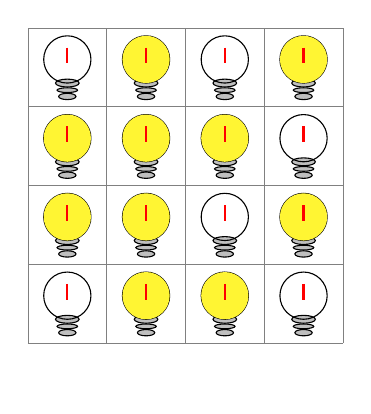
\begin{tikzpicture}[scale=1]
        \newif\ifbulbison\bulbisontrue
        
        \draw[step=1cm, gray, very thin] (0,0) grid (4,4);
        \tikzset{
            turned on/.is if=bulbison, 
            turned on/.default=true,
            light bulb/.style={
                path picture={       
                    % base (three ellipses)
                    \draw[fill=gray!50, draw=black] (0,0.1) ellipse (0.15 and 0.05);
                    \draw[fill=gray!50, draw=black] (0,0.01) ellipse (0.13 and 0.03);
                    \draw[fill=gray!50, draw=black] (0,-0.07) ellipse (0.11 and 0.04);
                    %circle
                    \draw[black] (0,0.4) circle (0.3);
                    % turned on
                    \ifbulbison
                        \fill[yellow!80!white] (0,0.4) circle (0.3);
                    \fi
                     % filament
                    \draw[thick, red] (0,0.55) -- (0,0.35);
                },
                minimum width=0.7cm,
                minimum height=1.5cm,
            }
        }
    
        % (x,y) -> (x - .5, y - .8)
        \foreach \x/\y in {1/1, 4/1, 3/2, 4/3, 1/4, 3/4} {
            \node[light bulb, turned on = false] at (\x - 0.5,\y - 0.8) { };
        }
        
        \foreach \x/\y in { 2/1, 3/1, 1/2, 2/2, 4/2, 1/3, 2/3, 3/3, 2/4, 4/4} {
            \node[light bulb, turned on = true] at (\x - 0.5,\y - 0.8) { };     
        }
    \end{tikzpicture}
    \end{center}
    \end{minipage}
\end{problem}

\begin{solution}[No, we can't.]
    The key with problems like these is often to focus on specific grid squares, rather than the whole. In the case of this problem, observe that 3 of the corners are off, and 1 is on. But, importantly, we cannot switch the state of one corner without toggling on/off exactly one other (for example, if you turn on the top left, you either turn on the bottom left or instead turn off the top right). Thus, if we consider just the 4 corners, every transformation changes the number of bulbs that are turned on by $0$, $2$, or $-2$. But since we start from $1$ turned on bulb, it is impossible to have all 4 corners on at once. And because of this, it is certainly impossible to turn on all 16 bulbs.
\end{solution}

\begin{problem}[C][3][A Walk Through Combinatorics]
    %Discrete ^ Pigeon-Hole Principle
    The set $M$ consists of nine positive integers, none of which has a prime divisor larger than six. Prove that $M$ has two elements whose product is the square of an integer.
\end{problem}

\begin{solution}
    % mine\\-matthew
    Since no integer $m \in M$ can have a prime factor other than 2, 3, or 5, they must all be of the form $m_i = 2^{a_i}3^{b_i}5^{c_i}$. Accordingly, the product $P = m_i \cdot m_j$ must be of the form $P_{i,j}=2^A 3^B 5^C$, where $(A,B,C)=(a_i+a_j,\, b_i+b_j,\, c_i+c_j)$. For $P_{i,j}$ to be a perfect square, we must have that $A,B,C$ are all even (for example, we know $2^6 3^0 5^2$ is perfect square because it can be written as $\left[ 2^3 3^0 5^1 \right]^2 = 40^2$). This means that the corresponding exponents of $m_i$ and $m_j$ must either both be even or both be odd, so that they sum to an even number. In other words, each pair $(a_i, a_j)$, $(b_i, b_j)$, and $(c_i, c_j)$ must having matching parity (both even or both odd) get an even $A,B$, and $C$. Since there are 3 exponents ($a_i, b_i, \text{and}\ c_i$) and each exponent has two possibilities (even or odd), there are $2^3=8$ combinations. But since $M$ has 9 elements, we can call on the Pigeonhole Principle to conclude that we'd be able to find at least 1 pair of elements where the corresponding exponents match in parity, and thus whose product is a perfect square. $\Box$
\end{solution}

\begin{problem}[C][5][BAMO 2013/4]
    % Construction ^ Invariants
    For a positive integer $n \geq 2$, consider the $n-1$ fractions
    $$ \frac{2}{1}, \frac{3}{2}, \ldots, \frac{n}{n-1}$$
    The product of these fractions equals $n$, but if you reciprocate (i.e. turn upside down) some of the fractions, the product will change. Can you make the product equal 1? Find all values of $n$ for which this is possible, and prove that you have found them all.
\end{problem}

\begin{solution}
    A few ideas come to mind as to how we might solve this---perhaps it relies on prime factorization, for example---but the solution is not immediately obvious. To start, then, we'll try a few examples. For $n=2$ and $n=3$, it doesn't seem to be possible. But for $n=4$, we can do
    \[
        \mathbf{\frac{2}{1}}\cdot\frac{3}{2}\cdot\frac{4}{3} 
        \quad \rightarrow \quad 
        \mathbf{\frac{1}{2}}\cdot\frac{\bcancel{3}}{2}\cdot\frac{4}{\bcancel{3}} 
        = 1.
    \]
    Unfortunately, $n=5$ doesn't seem to work, nor does $n=6$. Considering what's special about $n=4$ as opposed to these other numbers, notice that it's a perfect square. So we jump to $n=9$ and find that we can do
\[
    \mathbf{\frac{2}{1}\cdot\frac{3}{2}}\cdot\frac{4}{3}\cdot\frac{5}{4}\cdot\frac{6}{5}\cdot\frac{7}{6}\cdot\frac{8}{7}\cdot\frac{9}{8}
    \quad \rightarrow \quad
    \mathbf{\frac{1}{\cancel{\mathbf{2}}}\cdot\frac{\cancel{\mathbf{2}}}{3}} \cdot \frac{\bcancel{4}}{3} \cdot \frac{\cancel{5}}{\bcancel{4}} \cdot \frac{\bcancel{6}}{\cancel{5}} \cdot \frac{\cancel{7}}{\bcancel{6}} \cdot \frac{\bcancel{8}}{\cancel{7}} \cdot \frac{9}{\bcancel{8}} = 1.
\]
It seems, then, that it works whenever $n$ is a perfect square, in which case, to get a product of 1, we flip fractions until we reach the one with numerator $\sqrt{n}$. We'll formalize this with the following claim.

\textbf{Claim:} If $n=k^2$ for some $k\in\mathbb{Z}$, then it is possible to reach a product of 1.

\underline{Proof:} Suppose there's an integer $k$ such that $n=k^2$. Then we can write our $n$th product as
\[
\underbrace{\frac{2}{1} \cdot \frac{3}{2} \cdot \frac{4}{3} \cdots \frac{k-1}{k-2} \cdot \frac{k}{k-1}}_{\text{$R$}} \cdot \underbrace{\frac{k+1}{k} \cdot \frac{k+2}{k+1} \cdots \frac{n}{n-1}}_{\text{$S$}},
\]
and group it into smaller products $R$ and $S$ as shown above. $R$ is the product of all fractions with a numerator less than or equal to $k$, and $S$ is the product of all fractions with a numerator greater than $k$.

Now, observe that $\displaystyle R=\frac{k!}{(k-1)!} = k$ and $\displaystyle S=\frac{n!/k!}{(n-1)!/(k-1)!} = \frac{n}{k}$.

Thus, if we flip all the fractions in $R$, we achieve the desired product of
\[
    \frac{1}{R} \cdot S = \frac{1}{k} \cdot \frac{n}{k} = \frac{n}{k^2} = 1.
\]
But this is only half of our solution, because we need to show $n=k^2$ is the only case where it's possible to do this.

\textbf{Claim:} If it's possible to reach a product of 1 for $n$, we must have $n=k^2$.%for some $k\in\mathbb{Z}$

\underline{Proof:} We want to represent the fraction flipping algebraically. Observe that we can do this by multiplying our original product $n$ by the reciprocal of a given fraction twice---once to remove the unflipped fraction (recall that multiplying a fraction by its reciprocal gives 1), and again to insert the flipped fraction into the product. This means the product after fraction $r$ is flipped is $n\cdot(1/r)^2$, and the product after fractions $R=r_1r_2r_3\dots$ are flipped is $n\cdot(1/R)^2$. Since we're assuming that we can reach a product of 1, we now have
\[
    n\cdot(1/R)^2 = 1 \quad \Rightarrow \quad n=R^2.
\]
Note that if we had $R=\frac{a}{b}$ where $a,b$ were coprime and $b\neq1$---that is, if $R$ was not an integer---then $a^2,b^2$ would be coprime and $b^2\neq1$, so $R^2=\frac{a^2}{b^2}$ would not be an integer. But since $R^2=n\in\mathbb{Z}$, $R$ must be an integer and therefore $n$ is a perfect square. Note that we specifically get $R=\sqrt{n}$ which is consistent with the rest of our proof.

Finally, we've shown that it's possible to get a product of 1 if and only if $n$ is a perfect square. $\Box$
\end{solution}

\begin{problem}[C][8][Mock Spain 2025/2]
    %Chinese Remainder Theorem ^ Construction ^ Pigeon-Hole Principle
    Let $m$ be a positive integer. We say an integer $x$ is $m$-good if $a^m$ divides $x$ for some integer $a>1$. We say that an integer $x$ is $m$-bad if $x$ is not $m$-good. \smallbreak
    
    \begin{itemize}
        \item[a)] Is it true that for all integers $n>0$, there are $n$ consecutive integers that are $m$-bad? 
        \item[b)] Is it true that for all integers $n>0$, there are $n$ consecutive integers that are $m$-good? 
    \end{itemize}
\end{problem}

\begin{solution}[No and yes, respectively]
    The first part is false, to prove this claim we just need to find a particular integer $n$ for which a) fails. Simply take any $n \geq 2^m$; it is guaranteed that among $n$ consecutive integers, at least one of them is divisible by $2^m$. $\Box$

    As for the second part, we claim it is true. Let $2= p_1< p_2< \ldots <p_n$ be the first $n$ prime numbers and let $P = p_1p_2 \cdots p_n$. We know that the system of congruences 
    \begin{align*}
        x \equiv& -1 \pmod{p_1^m} \\
        x \equiv& -2 \pmod{p_2^m} \\
        \vdots& \\
        x \equiv& -n \pmod{p_n^m}
    \end{align*}
    has a solution $x$ under $\bmod{ \hspace{4pt} P^m}$. The existence of such $x$ means that $p_i^m \mid x + i$ for $i=1,2, \ldots, n$, and thus we are done $\Box$ 
\end{solution}

\section{Other Fun Stuff}\setcounter{problem}{0}

\begin{problem}[Z][2][AMATYC Fall 2015/13]
    % Knights and Knaves ^ Discrete
     Knights always tell the truth, and knaves always lie. A knight and $12N - 1$ other people (each one either a knight or a knave) sit in a circle, and each one says, “Exactly one of my two immediate neighbors is a knave.” How many knaves are in the circle?
 \end{problem}
\multOpt[5]{$2N$}[$3N$][$4N$][$6N$][Depends on $N$]

\begin{solution}[C]
    \begin{minipage}[t]{0.77\textwidth}
\vspace{-8pt}
Let $T$ represent a knight, and $F$ represent a knave. We know the original knight (A) is telling the truth, so he has one knight (B) and one knave (C) next to him. The neighboring knight (B) is also telling the truth, so he must be next to a knave on his other side. The neighboring knave (C) is lying, so he's either next to 2 knaves or 2 knights, the latter of which must be the case since he's already next to (A). As shown in the diagram, this pattern continues indefinitely, alternating between one knave and two knights (FTT). Thus, $1/3$ of the people in the circle will be knaves. In this case, that gives us $12N/3=\boxed{4N}$.
\end{minipage}%
\hfill
\begin{minipage}[t]{0.2\textwidth}
\vspace{-10pt}
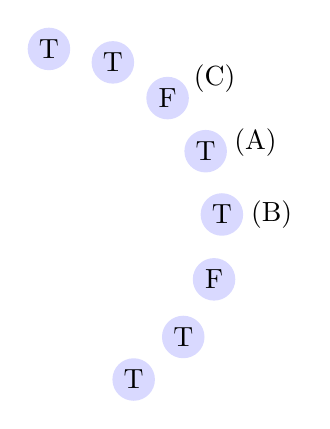
\begin{tikzpicture}[scale=1.5]
    \def\n{8}
    \pgfmathsetmacro{\N}{\n-1}
    \def\r{1.5}
    \def\labels{{"T", "T","F","T","T","F","T", "T"}}

    \foreach \i in {0,...,\N} {
        \coordinate (P\i) at ({\r*cos(170/\n*\i-60)}, {\r*sin(170/\n*\i-60)});
        \fill[blue!15] (P\i) circle (0.18cm);
        \node at (P\i) {\pgfmathparse{\labels[\i]}\pgfmathresult};
    }

    \node[yshift=3pt, xshift=18pt] at (P4) {(A)};
    \node[yshift=7pt, xshift=17pt] at (P5) {(C)};
    \node[xshift=18pt] at (P3) {(B)};
\end{tikzpicture}
\end{minipage}
\end{solution}

 \begin{problem}[Z][3]
    % Knights and Knaves ^ Discrete
    25 people are standing in a queue. Each of them is either a knight or a knave. The first person in the queue says that everybody behind them is a knave. Each of the others in the queue say that the person immediately in front of them in the queue is a knave.\\[\parskip]
    
    How many knights are in the queue?
 \end{problem}

 \begin{solution}[13]
    Let $P_n$ denote the $n$th person in the queue, where $P_1$ represents the person in front, and let $T$ denote a knight and $F$ denote a knave. 

    We first assume $P_1=T$ (i.e., that $P_1$ is a knight). But recall that $P_2$ claims $P_1=F$. So we conclude that $P_2=F$. Notice that this is exactly what $P_3$ claims, meaning $P_3=T$. But this contradicts $P_1=T$, since $P_1$ claimed everyone behind them was a knave. Thus we must instead have $P_1=F$. Then $P_2=T$, $P_3=F$, $P_4=T$, and so on, with the alternating pattern continuing until $P_{25}=F$. This gives us \fbox{12} knights in total.
 \end{solution}

 \begin{problem}[Z][3][BMT 2024 Discrete/7]
    % Counting ^ Discrete ^ Inclusion Exlusion Principle
     Gigi randomly rearranges four $G$’s and seven $I$’s to form an eleven-letter string. What is the probability that there is a group of four consecutive letters that form “$GIGI$,” her name?
 \end{problem}

 \begin{solution}[$2/5$]
     We can make a total of $\binom{4+7}{4} = 330$ eleven-letter strings using four $G$'s and seven $I$'s. Let $A_i$ be the event that positions $i, i+1, i+2$ and $i+3$ form the block "$GIGI$". We use the Inclusion-Exclusion Principle to count all the occurrences of "$GIGI$". First we count all cases in which there is at least one occurrence of the string "$GIGI$", we subtract all pairwise overlaps and then we add back all the triple overlaps.

    \textbf{At least one valid block:} If we fix an event $A_i$ for any $1 \leq i \leq 8$, then the remaining seven letters are made of two $G$'s and five $I$'s, this can be done in $\binom{2+5}{2} = 21$ ways, and we have 8 possible choices for $i$. Thus it adds up to $\sum |A_i| = 8 \cdot 21 = 168 $ 

    \textbf{Pairwise Overlaps} We count the cases where at least two "$GIGI$" blocks exist simultaneously. We look at the size of $A_i \cap A_j$ where $1 \leq i<j \leq 8$. It can be either two completely separated blocks---whenever $j-i \geq 4$---or they could be joined---whenever $j-i = 2$, the block $GIGIGI$. In the first case, the two separate blocks occupy 8 letters, the remaining letters are simply three $I$'s. For a fixed $A_i \cap A_j$, this can be done in just one way, and there are exactly 10 pairs where $j-i \geq 4$. In the second case, we make the six-letter block and the remaining letters are one $G$ and four $I$'s. For a fixed $A_i \cap A_j$ we can do so in $\binom{5}{1} = 5$ ways, and there are exactly 6 pairs where $j-i = 2$. 
    Thus $\sum |A_i \cap A_j | = 10 \cdot 1 + 6 \cdot 5 = 40$

    \textbf{Triple Overlap} It can also happen that three blocks of $GIGI$ occur together---that we find the eight-letter block "$GIGIGIGI$". We look at the size of $A_i \cap A_j \cap A_k$ where $1 \leq i < j < k \leq 8$ and $k-j =j - i = 2$, luckily, we don't have many of such cases. For a fixed triple overlap, we have to use all four $G$'s, so there is only one way to do it, and there are exactly 4 ways to fix the indices. Therefore the final case adds up to $\sum | A_i \cap A_j \cap A_k | = 4 \cdot 1 = 4$

    Putting all pieces together, our answer must be 
    \begin{align*}
        \sum_i |A_i| - \sum_{i < j} |A_i \cap A_j| + \sum _{i < j < k} |A_i \cap A_j \cap A_k | 
        = 168 - 40 + 4 = 132
    \end{align*}
     Recall that the total is 330, we obtain our desired probability as $132/330 = 2/5$ $\Box$  
 \end{solution}

 \begin{problem}[Z][3][BMT 2023 Discrete/3]
    % Counting
     Find the number of positive integers $n$ less than 10000 such that there are more 4’s in the digits of $n+1$ than in the digits of $n$.
 \end{problem}

\begin{solution}[1,111]
    To ensure that we get at least one more $4$'s in $n+1$ than in $n$, the digits of $n$ must end in a substring composed of one $3$ and $k$ $9$'s, where $0 \leq k \leq 3$.
    One valid example with $k=2$ is $7399$. Once we fix $k$ to ensure a valid $n$, we can select the other digits in $10^{3-k}$ different ways. Thus our answer is $1+10+10^2+10^3 = 1111$ $\Box$
\end{solution}

  \begin{problem}[Z][6][BMT 2024 Calculus/10]
    %Induction ^ Derivatives ^ Integrals
     Let a function \( f(n) \) satisfy \( f(1) = 0 \), and for positive integers \( n > 1 \),

    \[
    f(n) =
    \begin{cases}
    f\!\left(\frac{n}{2}\right) + \ln 2, & \text{if } n \text{ is even} \\
    \frac{f(n-1) + f(n+1)}{2}, & \text{if } n \text{ is odd}.
    \end{cases}
    \]
    
    Find the value of
    
    \[
    \lim_{n \to \infty} \frac{1}{2^n} \sum_{k=2^n}^{2^{n+1}} \big|\ln k - f(k)\big|.
    \]
 \end{problem}

 
\begin{solution}
    The first thing we may try is to open the absolute value, seeing for what values of $k$ is $\ln{k}-f(k)$ positive or negative, hoping for some elegant cancellation. I didn't find one, but it looks quite similar to a Riemann Sum. In fact, if we let $v = 2^n$ and make an index change to $r = k - v$, we get:
    $$\lim_{n \to \infty} \frac{1}{v} \sum_{r=0}^{v} \big|\ln ({v+r}) - f(v+r)\big|.$$
    After experimenting with the first values of $f(k)$. We can arrive to the next statement \smallbreak

    \textbf{Claim 1:} Let $v,k,r$ be integers such that $v$ is a power of 2, $k = v + r$ and  $0 \leq r <v \leq k < 2v$. Then 
    \begin{align}
          f(k) = \ln{v} +  \ln{2}\cdot \frac{r}{v}   \tag{ $\mathcal{T}$ } 
    \end{align}
    \underline{Proof:} We use strong induction with base case $f(1)=0$ given. Assuming that $(\mathcal{T})$ is true for any $k<K$, we will show that $(\mathcal{T})$ works for $k=K$ too.
    
    If $K$ is even, then $r = K - v$ is also even, and 
    \begin{align*}
        f(K) = \ln 2 + f \left( \frac{K}{2}\right) \overset{\mathcal{T}}{=} \ln 2 +  \ln \left( \frac{v}{2} \right) + \ln 2 \cdot \frac{r/2}{v/2} \\
        = \ln v + \ln 2 \cdot \frac{r}{v}
    \end{align*}
    Which works. Now if $K$ is odd, then $r = K - v$ is also odd, and both $K \pm 1$ are even
    \begin{align*}
        f(K) &= \frac{f(K-1) + f(K+1)}{2} = \frac{1}{2} \left( f\left( \frac{K+1}{2} \right) + f\left( \frac{K-1}{2} \right) + 2\ln 2\right ) \\
        &\overset{\mathcal{T}}{=} \ln 2 +  \frac{1}{2} \left( \ln \left( \frac{v}{2} \right) + \frac{(r-1)/2}{v/2} \cdot \ln 2  + \ln\left( \frac{v}{2} \right) + \frac{(r+1)/2}{v/2} \cdot \ln 2 \right) \\
        &= \ln 2 + \ln\left( \frac{v}{2} \right) + \frac{\ln 2}{2}\left( \frac{r-1}{v} + \frac{r+1}{v}   \right) = \ln{v} + \frac{r}{v} \cdot \ln 2
    \end{align*}
    So we conclude that $(\mathcal{T})$ is true in general $\Box$

    Using Claim 1, and the definition of Riemann Sum, we see that 
    \begin{align*}
          \lim_{n \to \infty} \frac{1}{v} \sum_{r=0}^{v-1} \left|\ln ({v+r}) - f(v+r) \right| &=
          \lim_{n \to \infty} \frac{1}{v} \sum_{r=0}^{v-1} \left| \ln(v+r) - \ln v - \ln 2 \cdot \frac{r}{v} \right| \\
          &= \lim_{n \to \infty} \frac{1}{v} \sum_{r=0}^{v-1} \left| \ln \left( 1 + \frac{r}{v} \right) - \ln2 \cdot \frac{r}{v}\right| \\
          &= \int_0^1 \big| \ln(1+x) - \ln2 \cdot x \big| \, \mathrm{d}x
    \end{align*}
    Note that when $r=v$, the expression $\ln k - f(k)$ is zero, so we can remove it and range $r$ in $[0,v-1]$.
    To get rid of the absolute value, we use the following statement: \smallbreak
    \textbf{Claim 2:} For $0 \leq x \leq 1$, we always have $\ln (1+x) \geq \ln 2 \cdot x$

    Proof: Let $h(x) = \ln(1+x) - \ln2 \cdot x$. Because $h'(x)$ has a unique zero $c = \frac{1}{\ln 2} - 1$, that lies within $[0,1]$, we know that $h(x)$ has at most two roots. By inspection, we can easily find that $h(0)=h(1)=0$ are these roots. Now we just test any value $0<x_0<1$ to see that $h(x_0)>0$, meaning that $h(x)>0$ for any $0<x<1$ and therefore  $\ln (1+x) \geq \ln 2 \cdot x$ $\Box$

    Now we just get rid of the absolute value and compute
    \begin{align*}
         \lim_{n \to \infty} \frac{1}{v} \sum_{r=0}^{v-1} \left|\ln ({v+r}) - f(v+r) \right| &=
         \int_0^1 [\ln(1+x) - \ln2 \cdot x] \, \mathrm{d}x \\
         &= (1+x) \ln (1+x) - x -  \ln2 \cdot \frac{x^2}{2} \bigg |_0^1 \\
         &= \frac{3}{2} \cdot \ln 2 - 1 
    \end{align*}
    $\Box$
\end{solution}

 
 %add calculas problem


\end{document}